\documentclass{ltjsarticle}

\title{CTRStation数学問題集}
\author{Bamboo}

\usepackage[luatex]{graphicx}
\usepackage{amsmath, amssymb}

\begin{document}

\maketitle

\begin{enumerate}
  \setlength{\parskip}{4cm}
  \everymath{\displaystyle}

  \item 図1の外側の円の半径が3のとき,三角形に内接する円の半径を求めよ.(Maru)

  \begin{figure}[htbp]
  \centering
  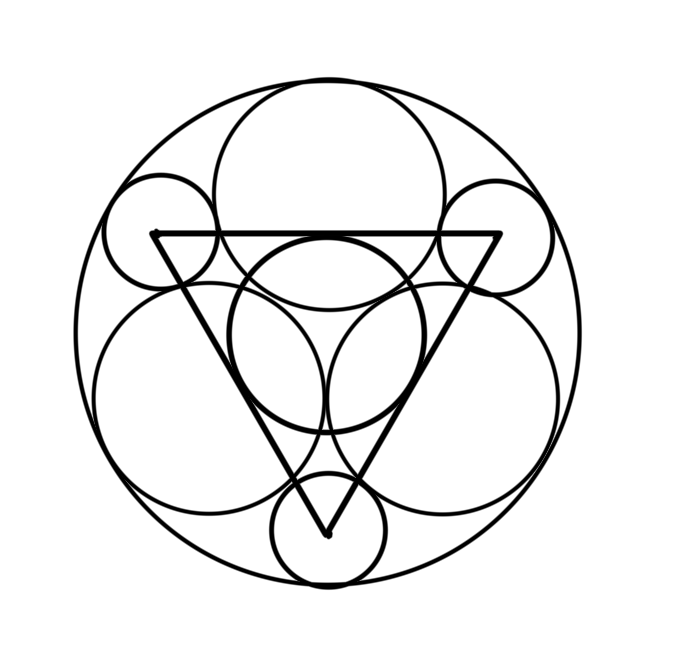
\includegraphics[scale=0.3]{radius.png}
  \caption{}
  \end{figure}

  \item 実数$t$が$0\le t\le1$を動くとき,放物線$y=x^2-\frac{1}{2}t^2x+\frac{1}{3}t^3$の通過領域を図示せよ.(Keito)
  \item 広義積分$\int_{0}^{∞}(x-a)^2be^{bx}\,dx$を求めよ.(Bamboo)
  \item $\sum_{n=1}^\infty \frac{1}{2^nn}$を求めよ.(Maru)
  \item $xy$平面における領域$D=\{(x,y)\,|\,x^2+y^2\le2y,\,x\ge0\}$の面積を求めよ.(Maru)

  \item $A=\begin{pmatrix}
    1 & 0 & -1 \\
    1 & -2 & 1 \\
    1 & -1 & 0
  \end{pmatrix}$について,
  \setlength{\parskip}{1.8cm}
  \begin{enumerate}
    \setlength{\parskip}{4cm}
    \item $A$の固有値を求めよ.
    \item $2\le n\in \mathbb{N}$のとき,$A^n$を求めよ.
  \end{enumerate}

  \setlength{\parskip}{4cm}

  \item $\int_{0}^{\pi}\frac{x}{\csc x(1+\cos ^2 x)}dx$を求めよ.(Bamboo)

\end{enumerate}

\end{document} 